% !TeX document-id = {f19fb972-db1f-447e-9d78-531139c30778}
% !BIB program = biber
\documentclass[compress]{beamer}
\usepackage[T1]{fontenc}
\usepackage{pifont}
\usetheme[block=fill,subsectionpage=progressbar,sectionpage=progressbar]{metropolis} 

\usepackage{wasysym}
\usepackage{etoolbox}
\usepackage[utf8]{inputenc}

\usepackage{threeparttable}
\usepackage{subcaption}

\usepackage{tikz-qtree}
\setbeamercovered{still covered={\opaqueness<1->{5}},again covered={\opaqueness<1->{100}}}


\usepackage{listings}

\lstset{
	basicstyle=\scriptsize\ttfamily,
	columns=flexible,
	breaklines=true,
	numbers=left,
	%stepsize=1,
	numberstyle=\tiny,
	backgroundcolor=\color[rgb]{0.85,0.90,1}
}



\lstnewenvironment{lstlistingoutput}{\lstset{basicstyle=\footnotesize\ttfamily,
		columns=flexible,
		breaklines=true,
		numbers=left,
		%stepsize=1,
		numberstyle=\tiny,
		backgroundcolor=\color[rgb]{.7,.7,.7}}}{}


\lstnewenvironment{lstlistingoutputtiny}{\lstset{basicstyle=\tiny\ttfamily,
		columns=flexible,
		breaklines=true,
		numbers=left,
		%stepsize=1,
		numberstyle=\tiny,
		backgroundcolor=\color[rgb]{.7,.7,.7}}}{}



\usepackage[american]{babel}
\usepackage{csquotes}
\usepackage[style=apa, backend = biber]{biblatex}
\DeclareLanguageMapping{american}{american-UoN}
\addbibresource{../../literature.bib}
\renewcommand*{\bibfont}{\tiny}

\usepackage{tikz}
\usetikzlibrary{shapes,arrows,matrix}
\usepackage{multicol}

\usepackage{subcaption}

\usepackage{booktabs}
\usepackage{graphicx}

\graphicspath{{../../pictures/}}

\makeatletter
\setbeamertemplate{headline}{%
	\begin{beamercolorbox}[colsep=1.5pt]{upper separation line head}
	\end{beamercolorbox}
	\begin{beamercolorbox}{section in head/foot}
		\vskip2pt\insertnavigation{\paperwidth}\vskip2pt
	\end{beamercolorbox}%
	\begin{beamercolorbox}[colsep=1.5pt]{lower separation line head}
	\end{beamercolorbox}
}
\makeatother



\setbeamercolor{section in head/foot}{fg=normal text.bg, bg=structure.fg}



\newcommand{\question}[1]{
	\begin{frame}[plain]
		\begin{columns}
			\column{.3\textwidth}
			\makebox[\columnwidth]{
				
\includegraphics[width=\columnwidth,height=\paperheight,keepaspectratio]{mannetje.png}}
			\column{.7\textwidth}
			\large
			\textcolor{orange}{\textbf{\emph{#1}}}
		\end{columns}
\end{frame}}


\title[ML in PYthon]{\textbf{A Practical Introduction to Machine Learning in Python} \\Day 4 -- Thursday \\ »Supervised Machine Learning«}
\author[Rupert Kiddle, Marieke van Hoof]{Rupert Kiddle \\ Marieke van Hoof \\ ~ \\ \footnotesize{r.t.kiddle@vu.nl, @rptkiddle \\ m.vanhoof@uva.nl, @marieke\_vh} \\}
\date{September 19, 2024}
\institute[Gesis]{Gesis}


\begin{document}
	
	\begin{frame}{}
		\titlepage
	\end{frame}
	
	\begin{frame}{Today}
		\tableofcontents
	\end{frame}
	
	

\section[Recap]{Recap: Top-down vs bottom-up}


\begin{frame}[plain]
\makebox[\linewidth]{
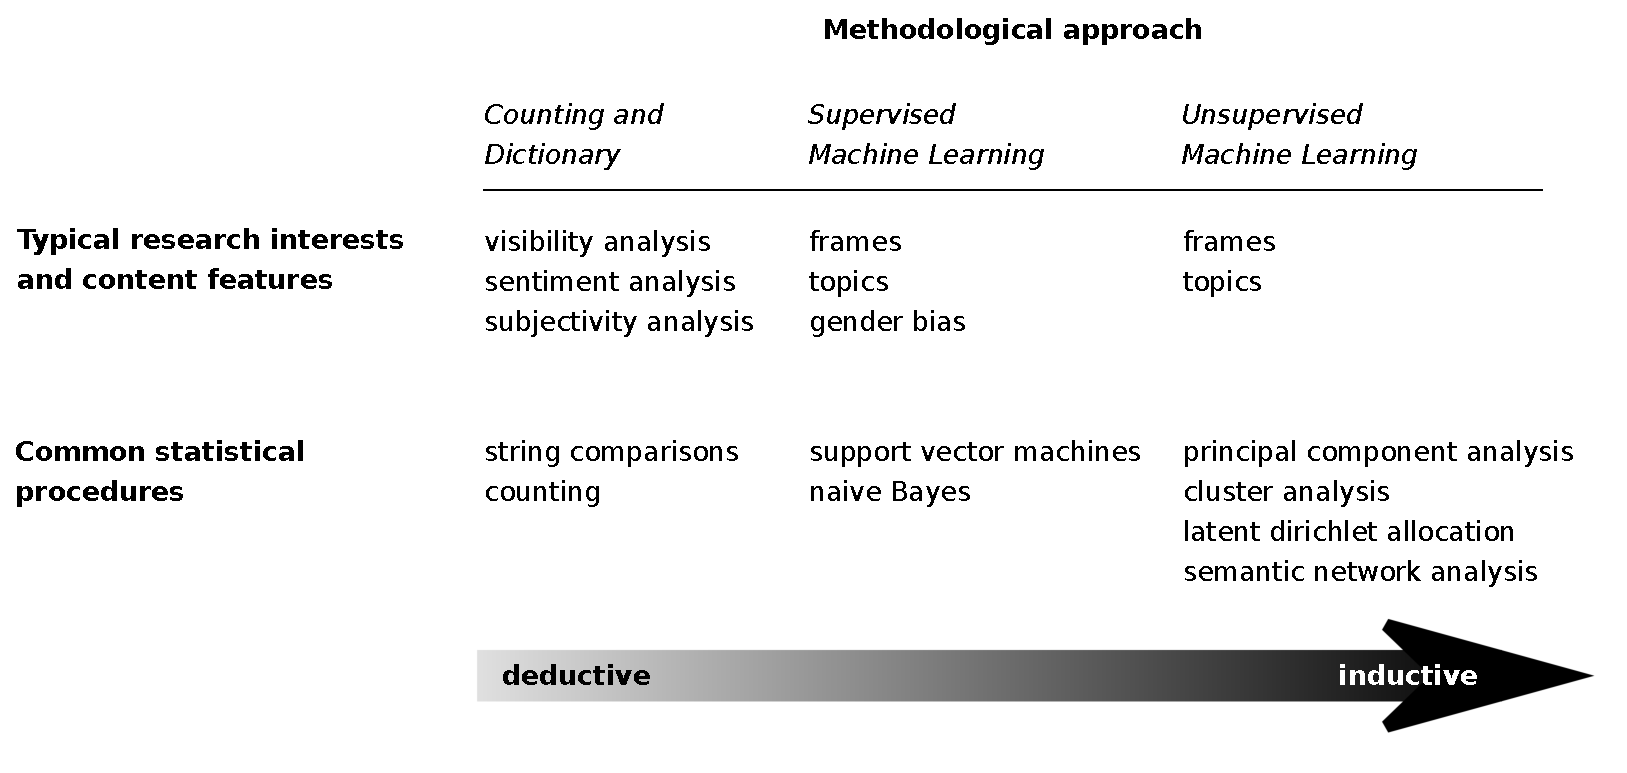
\includegraphics[width=\paperwidth,height=\paperheight,keepaspectratio]{boumanstrilling2016}}
\cite{Boumans2016}
\pause

%\textbf{\textcolor{orange}{The same logic applies to non-textual data!}}
\end{frame}
%}




\begin{frame}{Some terminology }
\begin{columns}[t]
\column{.5\textwidth}

\begin{block}<1-4>{Supervised machine learning}
You have a dataset with both predictor and outcome (independent and dependent variables; features and labels) --- a \emph{labeled} dataset.
\onslide<2>{
	\footnotesize{Think of regression: You measured \texttt{x1}, \texttt{x2}, \texttt{x3} and you want to predict \texttt{y}, which you also measured}}
\end{block}

\column{.5\textwidth}

\begin{block}<3->{Unsupervised machine learning}
You have no labels. \onslide<4>{(\footnotesize{You did not measure \texttt{y})}}\\
\onslide<5>{\textbf{Again, you already know some techniques to find out how \texttt{x1}, \texttt{x2},\ldots \texttt{x\_i} co-occur from other courses:} \begin{itemize}
		\item Principal Component Analysis (PCA) and Singular Value Decomposition (SVD)
		\item Cluster analysis
		\item Topic modelling (Latent Dirichlet Allocation)
		\item \ldots
	\end{itemize}
}
\end{block}

\end{columns}

\end{frame}




\section{Predicting things}






\subsection{You have done it before!}
\begin{frame}{You have done it before!}
	\begin{block}{Regression}<2->
		\begin{enumerate}
			\item<3-> Based on your data, you estimate some regression equation 	$y_i = \alpha + \beta_1 x_{i1} + \cdots + \beta_p x_{ip} + \varepsilon_i$
			\item<4-> Even if you have some \emph{new unseen data}, you can estimate your expected outcome $\hat{y}$!
			\item<5-> Example: You estimated a regression equation where $y$ is newspaper reading in days/week: $y = -.8 + .4 \times man + .08 \times age$
			\item<6-> You could now calculate $\hat{y}$ for a man of 20 years and a woman of 40 years -- \emph{even if no such person exists in your dataset}: \\
			$\hat{y}_{man20} = -.8 + .4 \times 1 + .08 \times 20 = 1.2$ \\
			$\hat{y}_{woman40} = -.8 + .4 \times 0 + .08 \times 40 = 2.4$
		\end{enumerate}
	\end{block}	
	
\end{frame}



\begin{frame}{}
	\huge{This is\\ Supervised Machine Learning!}
\end{frame}

\begin{frame}{\ldots but\ldots}
	\begin{itemize}
		\item<1-> We will only use \emph{half} {\tiny{(or another fraction)}} of our data to estimate the model, so that we can use the other half to check if our predictions match the manual coding (``labeled data'',``annotated data'' in SML-lingo)
		\begin{itemize}
			\item<2->e.g., 2000 labeled cases, 1000 for training, 1000 for testing --- if successful, run on 100,000 unlabeled cases
		\end{itemize}
		\item<3-> We use many more independent variables (``features'')
		\item<4-> Typically, IVs are word frequencies (often weighted, e.g. tf$\times$idf) ($\Rightarrow$BOW-representation)
	\end{itemize}
\end{frame}


\subsection{From regression to classification}
	
\begin{frame}[standout]
In the machine learning world, predicting some continous value is referred to as a \textcolor{orange}{regression} task. If we want to predict a binary or categorical variable, we call it a \textcolor{orange}{classification} task.

(quite confusingly, even if we use a logistic regression for the latter)
\end{frame}


\begin{frame}{Classification tasks}
For many computational approaches, we are actually not that interested in predicting a continuous value. Typical questions include:
\begin{itemize}
	\item Is this article about topic A, B, C, D, or E?
	\item Is this review positive or negative?
	\item Does this text contain frame F?
	\item Is this satire? 
	\item Is this misinformation?
	\item Given past behavior, can I predict the next click?
\end{itemize}
\end{frame}



\begin{frame}[plain]
	\begin{columns}[]
		\column{.5\textwidth}
		
		{\tiny{http://commons.wikimedia.org/wiki/File:Precisionrecall.svg}}
		\makebox[\linewidth]{
			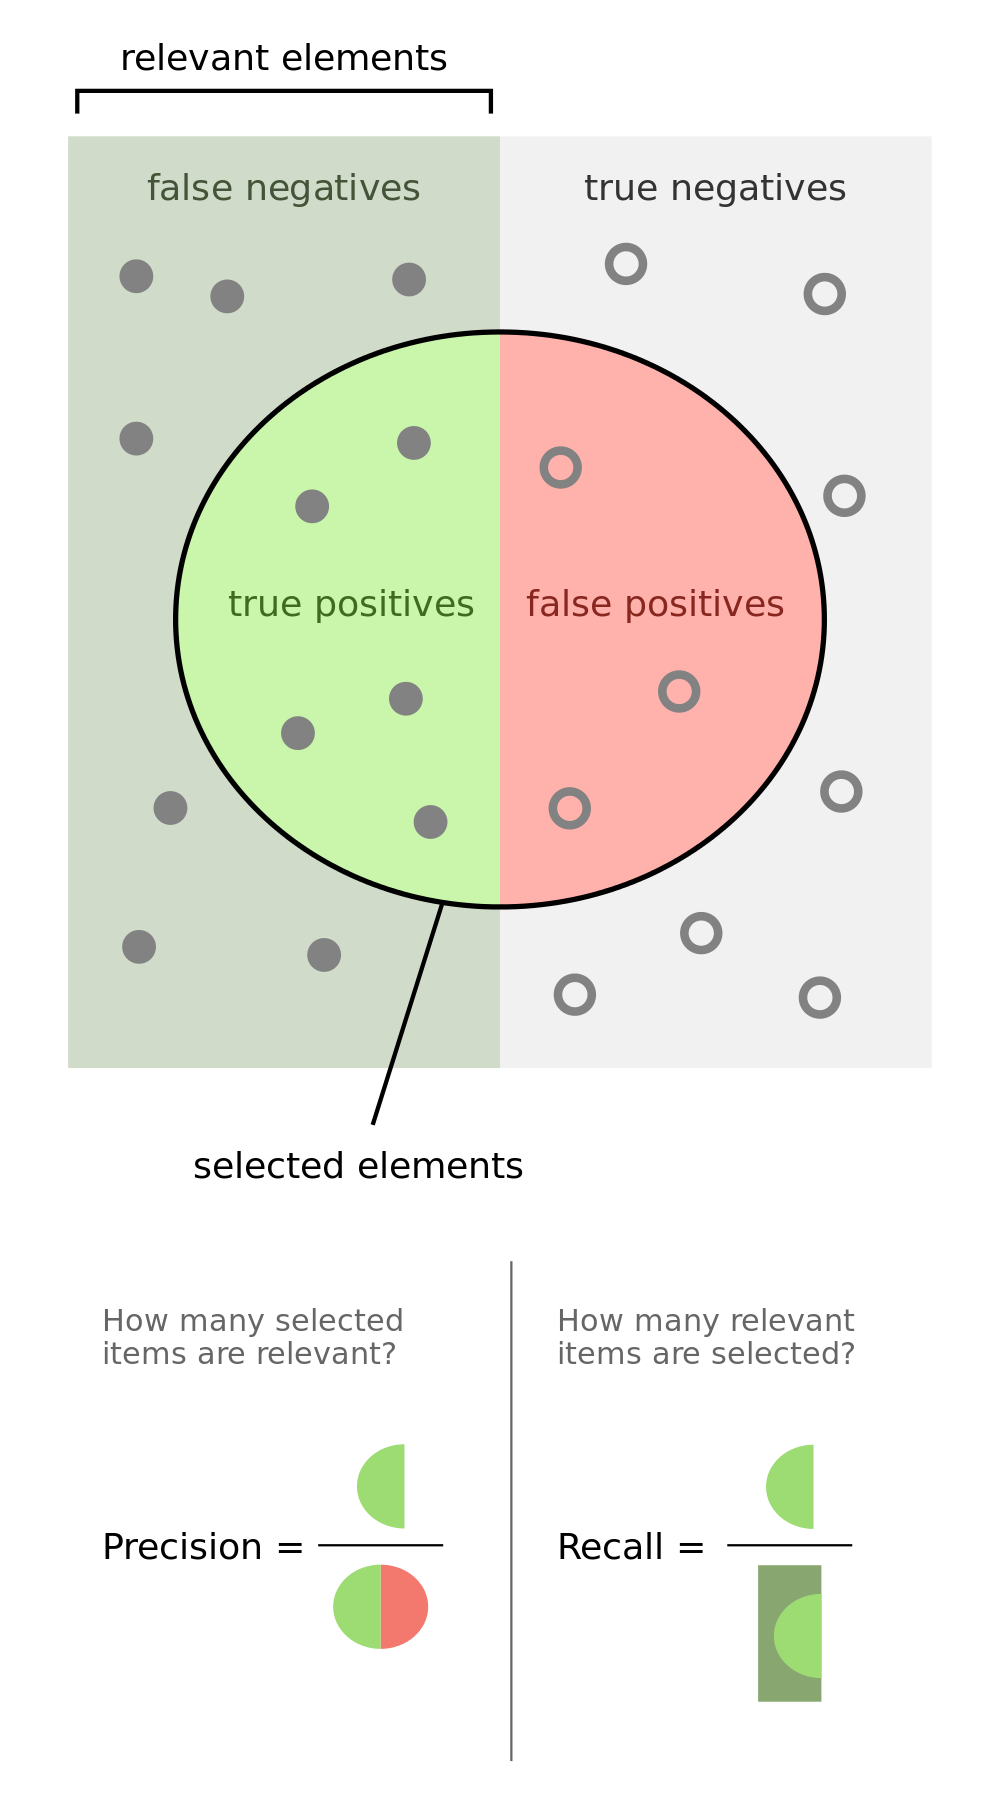
\includegraphics[width=\paperwidth,height=\paperheight,keepaspectratio]{../pictures/precisionrecall.png}}
		
		\column{.5\textwidth}
		\begin{block}{Some measures}
			\begin{itemize}
				\item Accuracy
				\item Recall
				\item Precision
				\item $\text{F1}=2\cdot \frac{\text{precision}\cdot \text{recall}}{\text{precision}+\text{recall}}$
				\item AUC (Area under curve) $[0,1]$, $0.5=$ random guessing
			\end{itemize}
		\end{block}
		
		
	\end{columns}
	
\end{frame}





\begin{frame}{Different classification algorithms}

\begin{itemize}[<+->]
	\item It is an empirical question which one works best
	\item We typically try several ones and select the best
	\item (remember: we have a test dataset that we did \emph{not} use to train the model, so that we can assess how well it predicts the test labels based on the test features)
	\item To avoid $p$-hacking-like scenario's (which we call ``overfitting''), there are techniques available (e.g., cross-validation, which we address this afternoon)
\end{itemize}
(to make it easier, imagine a binary classfication ("positive"/"negative"), but it doesn't really matter whether there are two or more labels)
\end{frame}






\begin{frame}{Naïve Bayes}
	\begin{block}{Bayes' theorem}
		$$ P(A \mid B) = \frac{P(B \mid A) \times P(A)}{P(B)} $$
	\end{block}
	\pause
	\textcolor{red}{A = Text is about sports\\
		B = Text contains `very', `close', `game'}.
	\pause
	Furthermore, we simply multiply the probabilities for the features:
	\textcolor{red}{$$P(B) = P(very\, close\, game) = P(very) \times P(close) \times P(game)$$}
	We can fill in all values by counting how many articles are about sports, and how often the words occur in these texts.
	\vspace{0.3cm}
	%\footnotesize{
	%	(Fully elaborated example on \url{https://monkeylearn.com/blog/practical-explanation-naive-bayes-classifier/})}
\end{frame}

\begin{frame}{Naïve Bayes}
	\begin{itemize}[<+->]
		\item It's ``naïve'' because the features are treated as completely independent ($\neq$ ``controlling'' in regression analysis)
		\item It's fast and easy
		\item It's a good \emph{baseline} for binary classification problems
	\end{itemize}
\end{frame}




\begin{frame}{Na\"ive Bayes}
$$ P(\rm{label} \mid \rm{features}) =$$
$$ \frac{P(x_1 \mid label) \cdot P(x_2 \mid \rm{label})\ \cdot P(x_3 \mid label) \cdot P(label)}{P(x_1) \cdot P(x_2) \cdot P(x_3)}$$.

	
\begin{itemize}
	\item Formulas always look intimidating, but we only need to fill in how many documents containing feature $x_n$ have the label, how often the label occurs, and how often each feature occurs
	\item Also for computers, this is \emph{really easy and fast}
	\item Weird assumption: features are independent
	\item Often used as a baseline
\end{itemize}
\end{frame}




\begin{frame}{Logistic Regression}
	\begin{block}{Probability of a binary outcome in a regression model}
		$$p = \frac{1}{1 + e^{-(\beta_0 + \beta_1 x_1 + \beta_2 x_2 + \ldots + \beta_n x_n)}}$$
	\end{block}
	Just like in OLS regression, we have an intercept and regression coefficients. 
	We use a threshold (default: 0.5) and above, we assign the positive label (`good movie'), below, the negative label (`bad movie').
\end{frame}
\begin{frame}{Logistic Regression}
	\begin{itemize}[<+->]
		\item The features are \emph{not} independent.
		\item Computationally more expensive than Naïve Bayes
		\item We can get probabilities instead of just a label
		\item That allows us to say how sure we are for a specific case
		\item \ldots or to change the threshold to change our precision/recall-trade off (e.g., 0.7 = higher precision, lower recall)
	\end{itemize}
\end{frame}

\begin{frame}{Support Vector Machines}
	\begin{columns}
		\column{.5\linewidth}
		\begin{itemize}
			\item	Idea: Find a hyperplane that best separates your cases
			\item Can be linear, but does not have to be (depends on the so-called kernel you choose)
			\item Very popular 
		\end{itemize}
		\column{.5\linewidth}	
		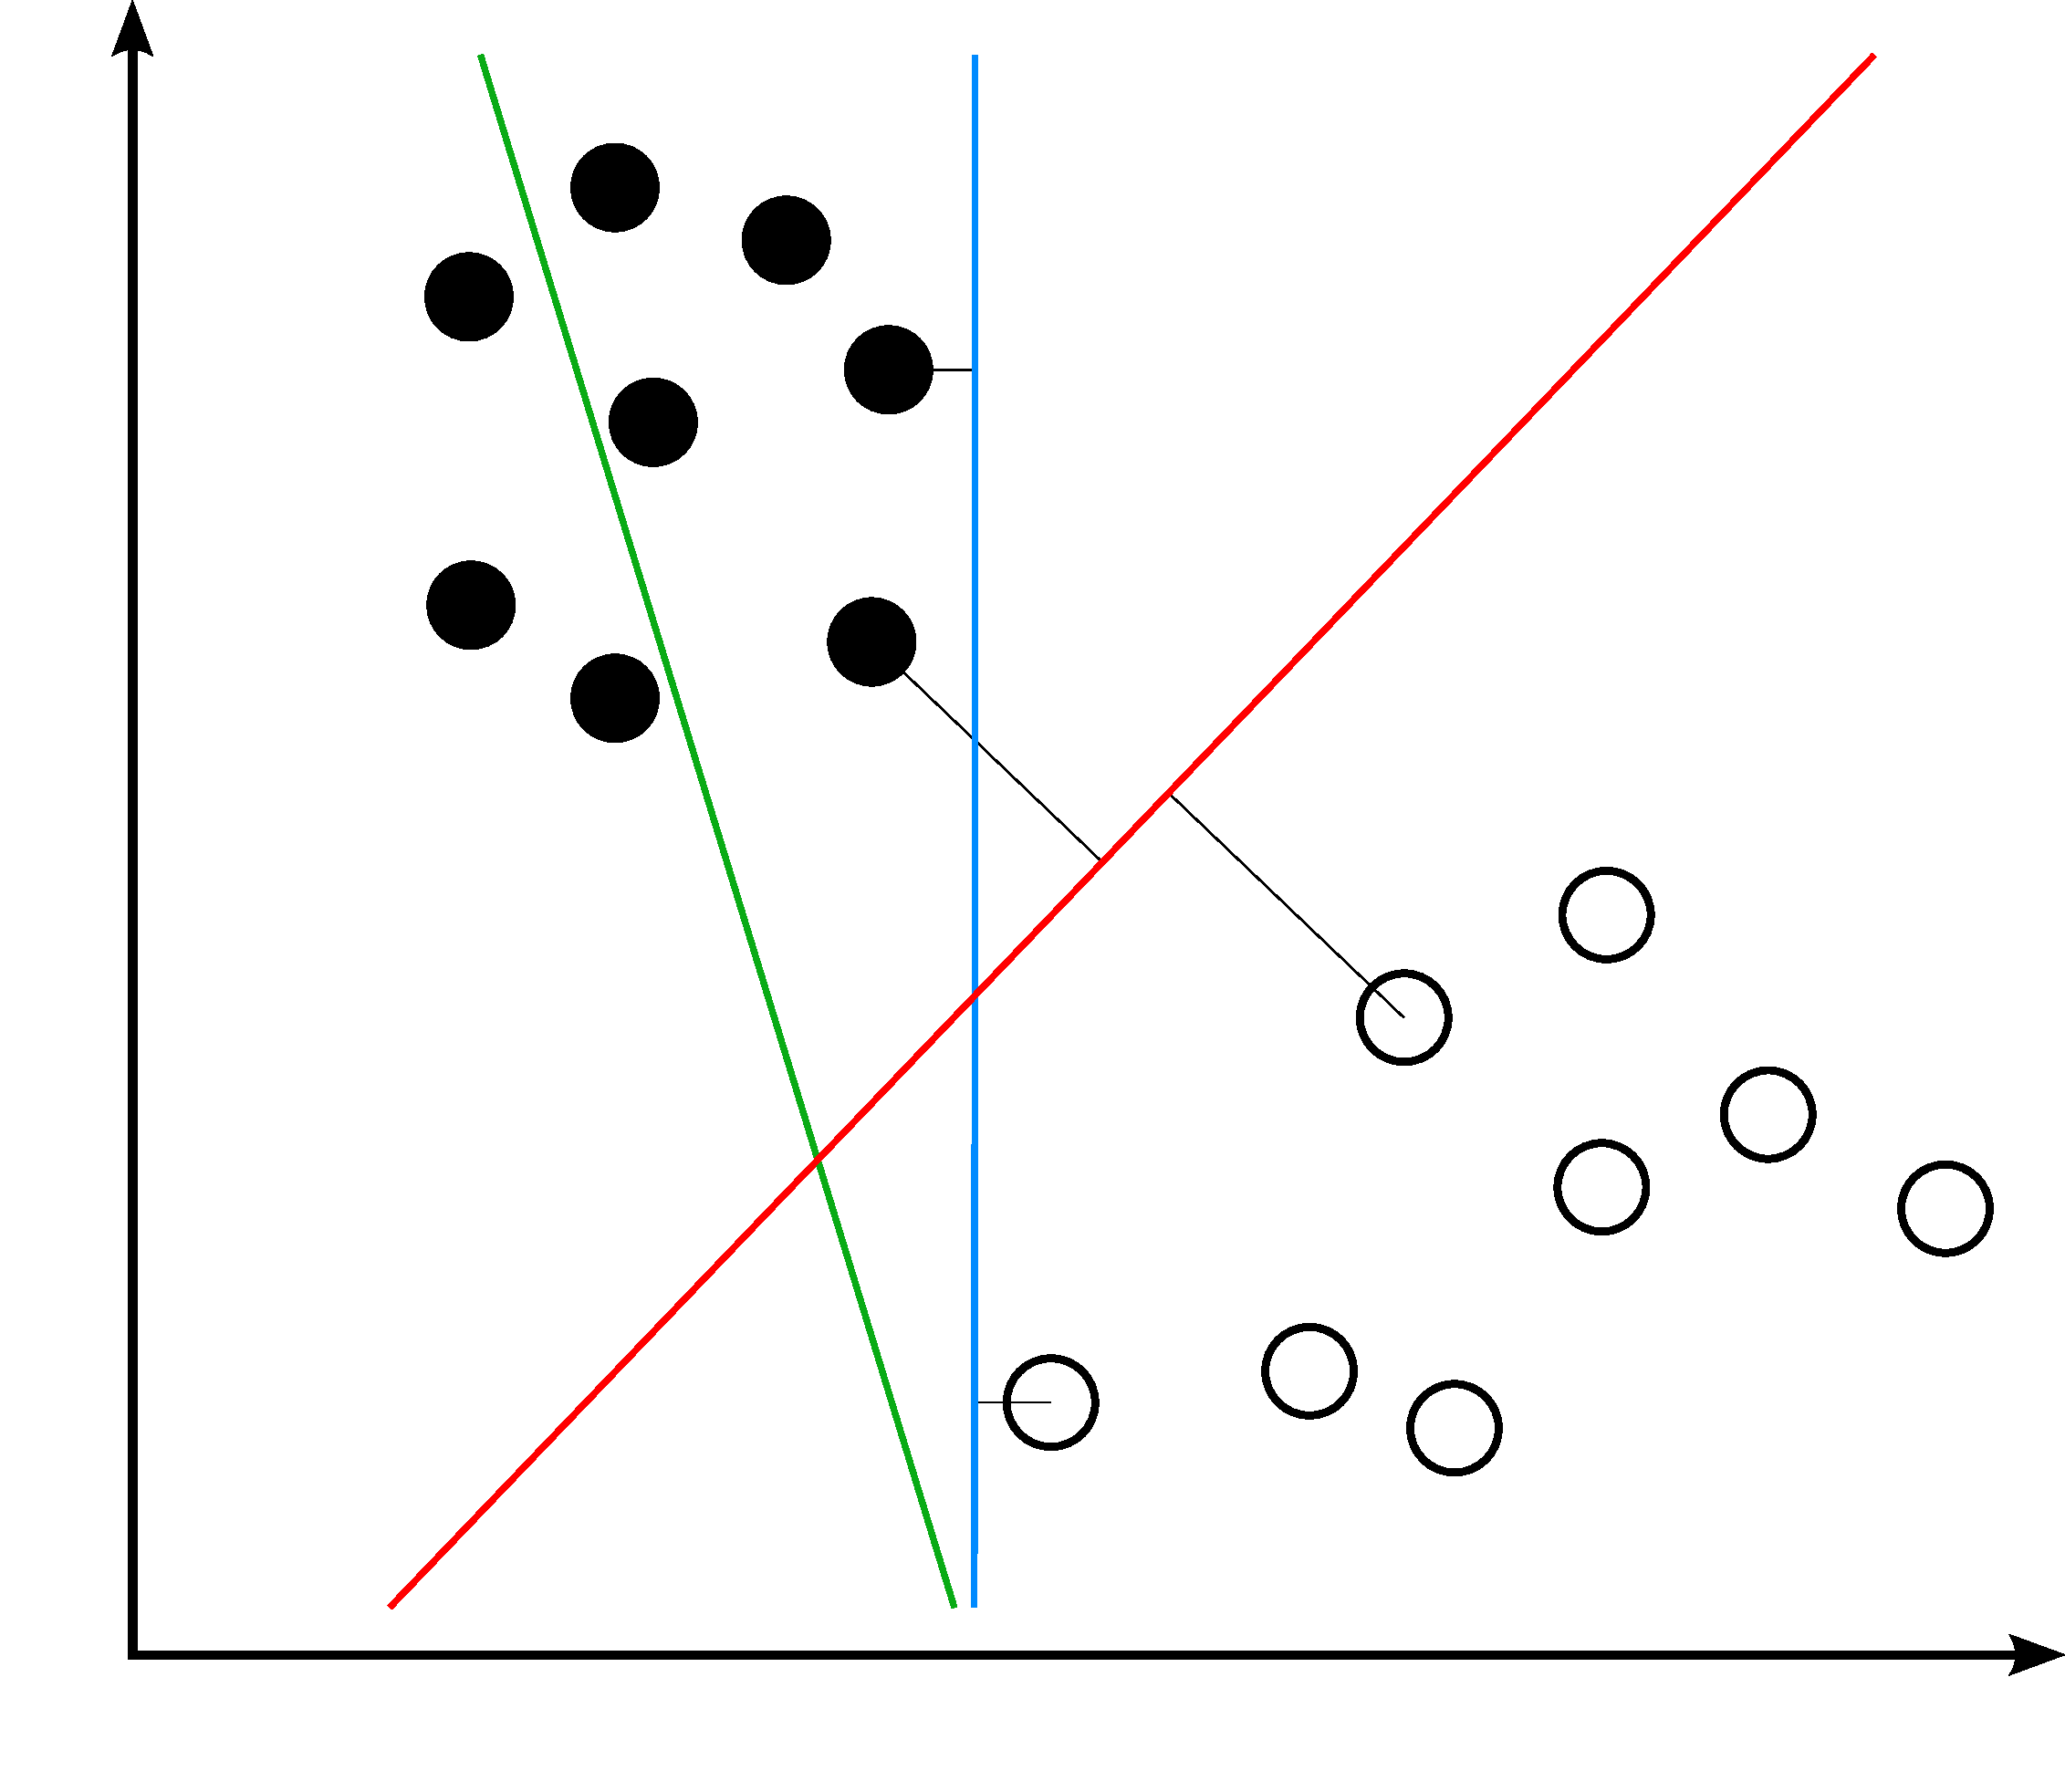
\includegraphics[width=.8\linewidth,height=.5\paperheight,keepaspectratio]{../pictures/svm}
		\tiny{\url{https://upload.wikimedia.org/wikipedia/commons/b/b5/Svm\_separating\_hyperplanes\_\%28SVG\%29.svg}}
	\end{columns}
	\vfill
	%\footnotesize{(Further reading: \url{https://monkeylearn.com/blog/introduction-to-support-vector-machines-svm/)}}
\end{frame}

\begin{frame}{SVM vs logistic regression}
\begin{itemize}
	\item for \emph{linearly separable} classes not much difference
	\item with the right hyperparameters, SVM is less sensitive to outliers
	\item biggest advantage: with the \emph{kernel trick}, data can be transformed that they \emph{become} linearly separable
\end{itemize}
\end{frame}


\begin{frame}{Decision Trees and Random Forests}
	\begin{columns}
		\column{.5\linewidth}
		\begin{itemize}[<+->]
			\item Model problem as a series of decisions (e.g., if cloudy then \ldots if temperature > 30 degrees then \ldots)
			\item Order and cutoff-points are determined by an algorithm
			\item Big advantage: Model non-linear relationships
			\item And: They are easy to interpret (!) (``white box'')
		\end{itemize}
		\column{.5\linewidth}	
		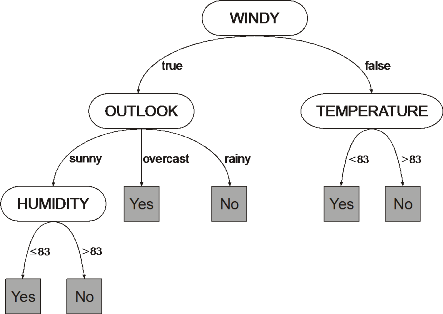
\includegraphics[width=.8\linewidth,height=.5\paperheight,keepaspectratio]{../pictures/decisiontree}
		\tiny{\url{https://upload.wikimedia.org/wikipedia/en/4/4f/GEP\_decision\_tree\_with\_numeric\_and\_nominal\_attributes.png}}
	\end{columns}
\end{frame}
\begin{frame}{Decision Trees and Random Forests}
	\begin{block}{Disadvantages of decision trees}
		\begin{itemize}
			\item comparatively inaccurate
			\item once you are in the wrong branch, you cannot go `back up'
			\item prone to overfitting (e.g., outlier in training data may lead to completely different outcome)
		\end{itemize}
	\end{block}
	\pause
	Therefore, nowadays people use \emph{random forests}: Random forests \emph{combine} the predictions of \emph{multiple} trees
	$\Rightarrow$ might be a good choice for your non-linear classification problem
\end{frame}






\section{Supervised Machine Learning for Text Classification}

\subsection{(Traditional) non-SML approaches}

\begin{frame}{Let's consider three tasks}
	For a given text (say, a news article, a press release, a review), determine the
	\begin{description}
		\item[sentiment] e.g., [positive|neutral|negative]
		\item[topic] e.g., [sports|economy|politics|entertainment|other]
		\item[frames] e.g., [economic|human|moral|conflict], or non-exclusive: economic = [0|1], human = [0|1], \ldots
	\end{description}
\end{frame}


%\question{What would be the strengths and weaknesses of different approaches for each of these tasks?}


\question{Imagine using a dictionary-based (list of keywords, list of regular expressions, or similar) approach to these tasks. How does the design (length, inclusiveness, etc.) of this list influence precision and recall?}


\begin{frame}{Dictionary-based approaches for text classification}
	\begin{columns}[t]
		\column{.5\textwidth}
		\begin{block}{good for}
			\begin{itemize}
				\item distinct, manifest things (names of organizations, pronouns, swearwords (?), \ldots)
				\item little room for interpretation/misunderstandings etc.
				\item ``must-be-explainable-to-a-five-year-old''
			\end{itemize}
			\pause
		\end{block}
		\column{.5\textwidth}
		\begin{alertblock}{bad for}
			\begin{itemize}
				\item latent constructs and concepts
				\item implicit things
			\end{itemize}
			\pause
			Hence, \emph{not} state-of-the-art for
			\begin{itemize}
				\item topics
				\item frames
				\item sentiment
			\end{itemize}
		\end{alertblock}
	\end{columns}
\end{frame}


\begin{frame}{From dictionary approaches to SML}
	\begin{itemize}[<+->]
		\item Early days of sentiment analysis: list of positive words, list of negative words, count what occurs most
		\item You can even \textit{buy} lists of words that are meant to measure constructs like ``positive emotions'' or even ``analytic'' or ``authentic'' language use from a psychologist (LIWC, \cite{Pennebaker2007})
	\end{itemize}
\end{frame}

\question{What do you think? Can this even work?}





\begin{frame}{Bag-of-words dictionary approaches to sentiment analysis}
	\begin{block}{con}
		\begin{itemize}
			\item simplistic assumptions
			\item e.g., intensifiers cannot be interpreted (``really'' in ``really good'' or ``really bad'')
			\item or, even more important, negations.
		\end{itemize}
	\end{block}
\end{frame}




\begin{frame}{Improving the BOW approach}
	\begin{block}{Example: Sentistrenght \parencite{Thelwall2012}}
		\begin{itemize}
			\item $-5\ldots-1$ and $+1\ldots+5$ instead of positive/negative
			\item spelling correction
			\item ``booster word list'' for strengthening/weakening the effect of the following word
			\item interpreting repeated letters (``baaaaaad''), CAPITALS and !!!
			\item idioms
			\item negation 
		\end{itemize}
	\end{block}
	
	VADER by \cite{Hutto2014} works in a similar way.
	\pause
	\footnotesize{Even though this is much less na\"ive than LIWC, for instance, the problem remains: Can we construct a dictionary that, \emph{irrespective of the context}, gives us a meaningful estimate of sentiment? }
\end{frame}





\begin{frame}[standout]
	Such an \textit{off-the-shelf} dictionary does not (and probably cannot) exist.
\end{frame}



\begin{frame}{\cite{Boukes2020}: Sentiment analysis of economic news}
	\makebox[\columnwidth]{
		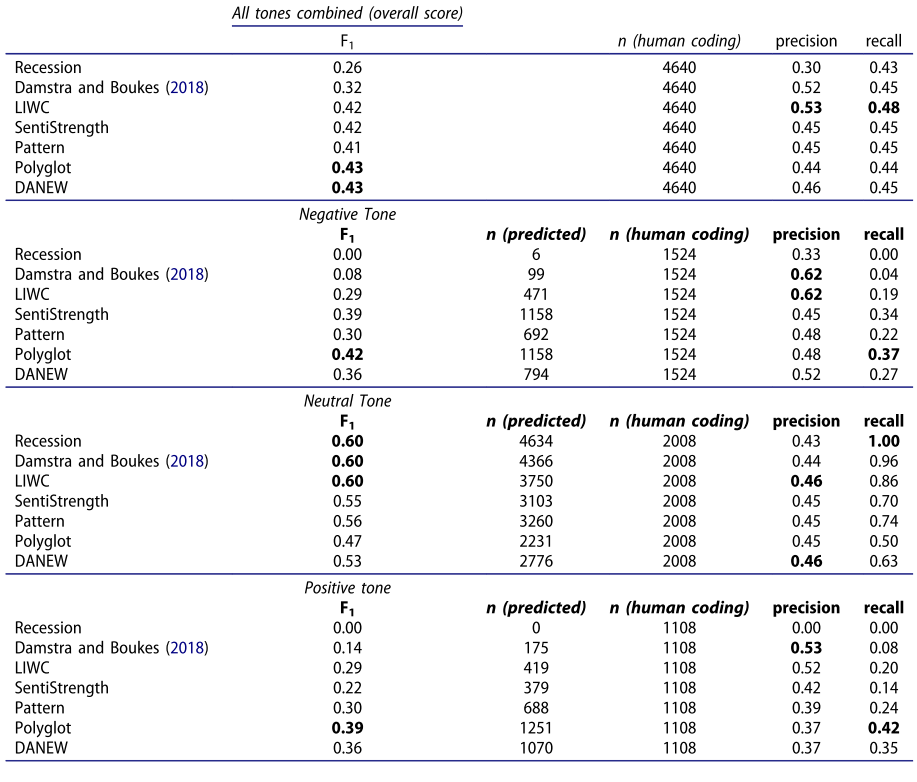
\includegraphics[width=\columnwidth,height=.8\paperheight,keepaspectratio]{boukes2019}}
\end{frame}


\begin{frame}{\cite{Boukes2020}: Sentiment analysis of economic news}
	\makebox[\columnwidth]{
		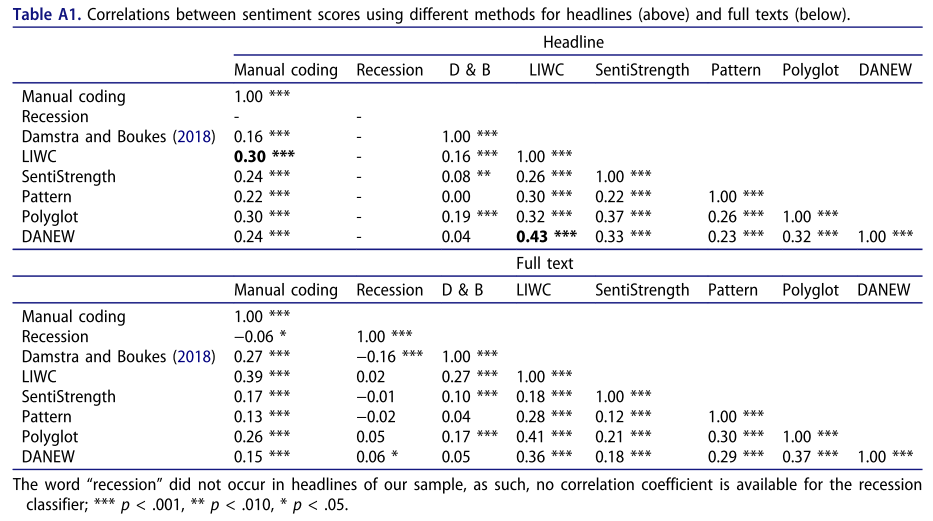
\includegraphics[width=\columnwidth,height=.8\paperheight,keepaspectratio]{boukes2019b}}
\end{frame}


\begin{frame}{\cite{Boukes2020}: Sentiment analysis of economic news}
	\begin{itemize}
		\item Dictionaries have low agreement with each other, and also with human coders
		\item Even their own dictionary didn't agree
		\item \textbf{This is not because these dictionaries are particularly bad!} Main point: For such a complex and context-dependent task, a dictionary is just not the right tool.
	\end{itemize}
\end{frame}




\begin{frame}{\cite{VanAtteveldt2021}: Extending \cite{Boukes2020} with SML}
	``manual coding (using undergraduate students) yields the
	best results 
	
	[\ldots] A good second place is taken by crowd coding [\ldots]  
	
	
	[\ldots] machine learning performs worse than both students' manual coding and crowd coding.
	Reaching $\alpha = 0.50$ for deep learning (CNN) and slightly worse for classical machine learning (SVM; $\alpha = 0.41$, NB; $\alpha = 0.40$), machine learning still performs significantly better than chance. However, since these results are lower than generally accepted levels of inter-coder reliability [\ldots]
	
	Finally, [\ldots] dictionaries [\ldots] perform worse than the machine
	learning results and much worse than manual annotation [\ldots] [and] approximate chance agreement''\end{frame}






\begin{frame}{\cite{Vermeer2019}: Satisfaction with brands}
	\makebox[\columnwidth]{
		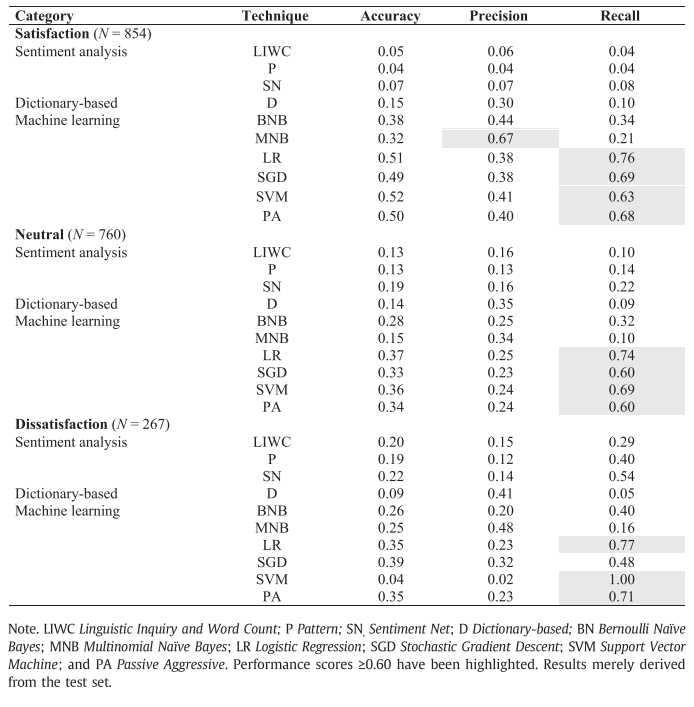
\includegraphics[width=\columnwidth,height=.8\paperheight,keepaspectratio]{vermeer2019}}
\end{frame}



\begin{frame}[standout]
	SML is no panacea, but the most promising approach to analyzing large quantities of texts. Don't believe off-the-shelf packages that claim to do the work for you.
	(For small datasets, just do it by hand.)
\end{frame}




\subsection{Diving into SML}




\begin{frame}{SML to code frames and topics}
	\begin{block}{Some work by \cite{Burscher2014} and \cite{Burscher2015} }
		\begin{itemize}
			\item Humans can code generic frames (human-interest, economic, \ldots)
			\item Humans can code topics from a pre-defined list 
			\item<2->\textbf{But it is very hard to formulate an explicit rule} \\(as in: code as 'Human Interest' if regular expression R is matched)
		\end{itemize}
		\onslide<3>$\Rightarrow$ This is where you need supervised machine learning!
	\end{block}
	
	
\end{frame}




{\setbeamercolor{background canvas}{bg=black}
	\begin{frame}[plain]
		\makebox[\linewidth]{
			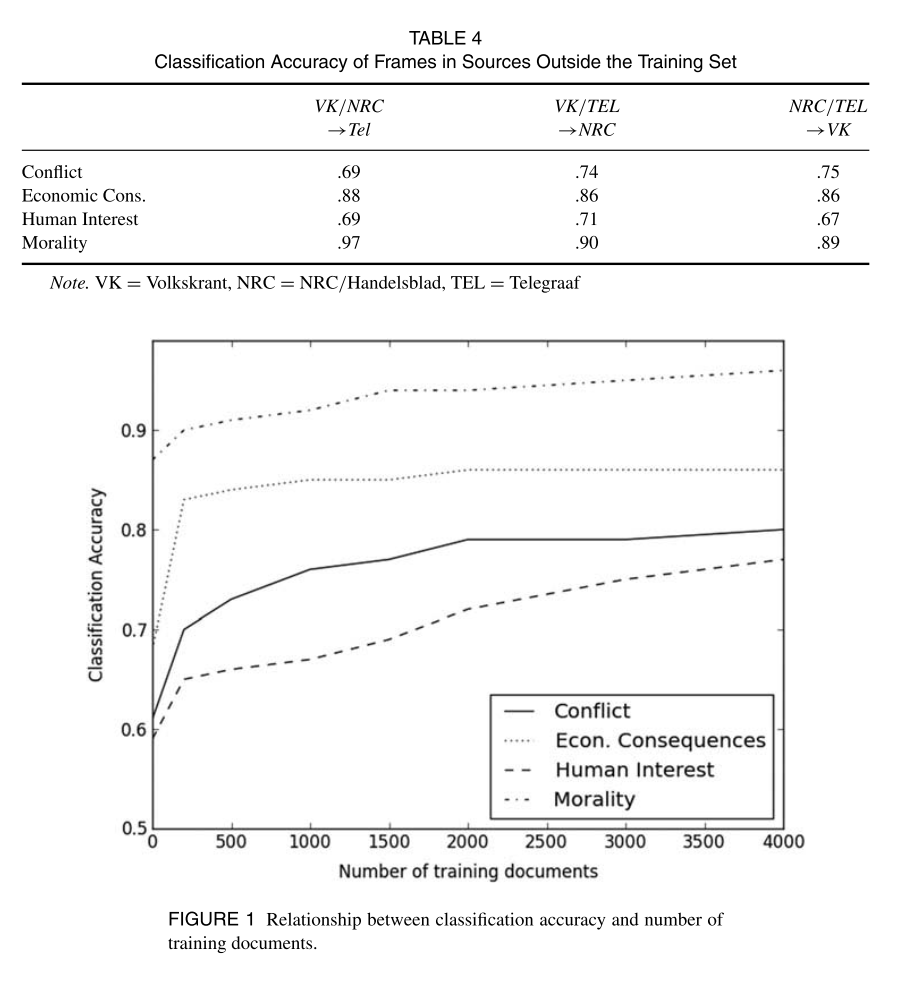
\includegraphics[width=\paperwidth,height=\paperheight,keepaspectratio]{burscher2014}}
	\end{frame}
	
	\begin{frame}[plain]
		\makebox[\linewidth]{
			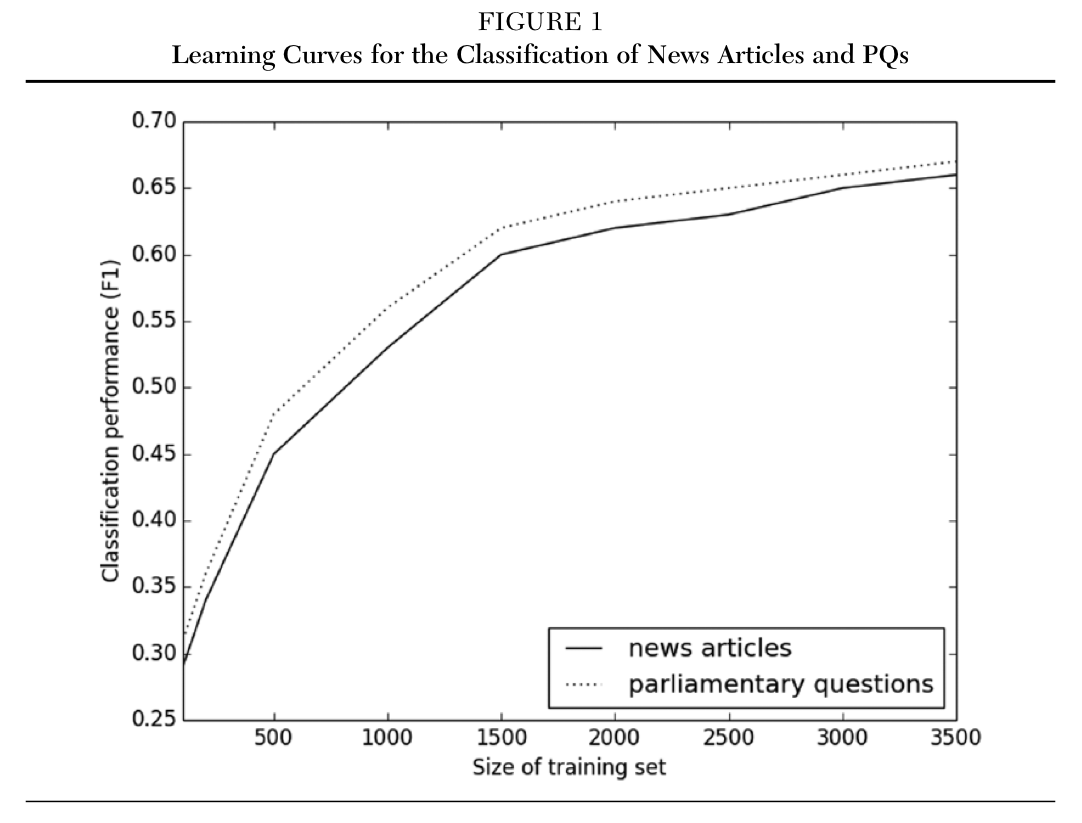
\includegraphics[width=\paperwidth,height=\paperheight,keepaspectratio]{burscher2015-a}}
	\end{frame}
	
	\begin{frame}[plain]
		\makebox[\linewidth]{
			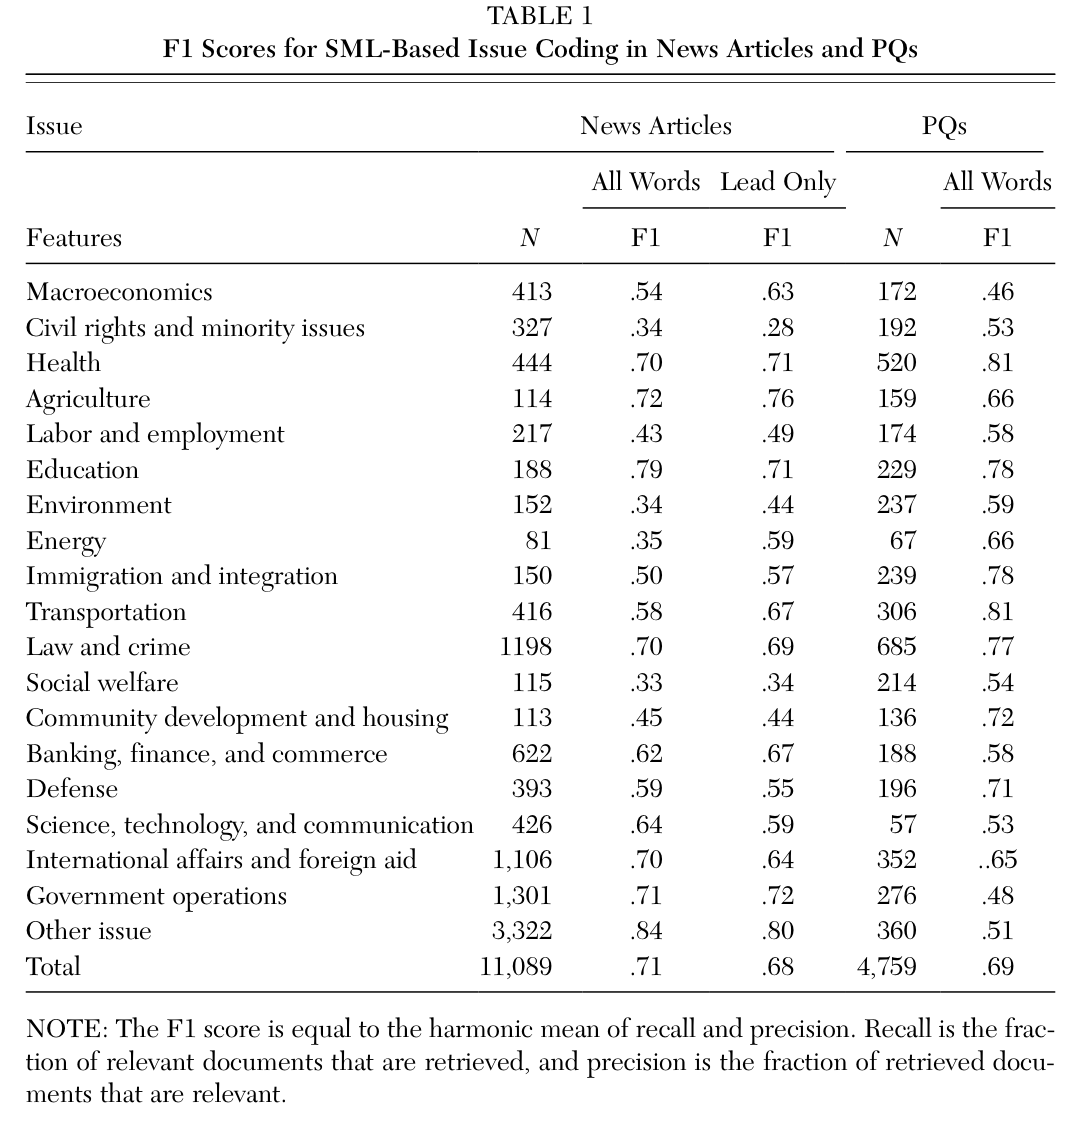
\includegraphics[width=\paperwidth,height=\paperheight,keepaspectratio]{burscher2015-b}}
	\end{frame}
}





\begin{frame}{What does this mean for our research?}
	\begin{block}<2>{It we have 2,000 documents with manually coded frames and topics\ldots}
		\begin{itemize}
			\item we can use them to train a SML classifier
			\item which can code an unlimited number of new documents
			\item with an acceptable accuracy (at least for some of them)
		\end{itemize}
	\end{block}
	\onslide<2>{
		\tiny{Some easier tasks even need only 500 training documents, see \cite{Hopkins2010}}}.
\end{frame}



\subsection{An implementation}

\begin{frame}[fragile]{An implementation}
Let's say we have two lists, with movie reviews and their rating:
\begin{lstlisting}
reviews_train = ["This is a great movie", "Bad movie", ... ...]
labels_train = [1,-1, ...]  
\end{lstlisting}
And a second dataset with an identical structure:
\begin{lstlisting}
reviews_test = ["Not that good","Nice film", ... ...]
labels_text = [-1,1, ......]
\end{lstlisting}
Both are drawn from the same population, it is pure chance whether a specific review is on the one list or the other.\\
\tiny{Based on an example from \url{http://blog.dataquest.io/blog/naive-bayes-movies/}}
\end{frame}

\begin{frame}[fragile]{Training a A Naïve Bayes Classifier}
  \begin{lstlisting}
from sklearn.naive_bayes import MultinomialNB
from sklearn.feature_extraction.text import CountVectorizer
from sklearn import metrics

vectorizer = CountVectorizer(stop_words='english')
features_train = vectorizer.fit_transform(reviews_train)
features_test = vectorizer.transform(reviews_test)

# Fit a naive bayes model to the training data.
nb = MultinomialNB()
nb.fit(features_train, labels_train)

# Now we can use the model to predict classifications for our test features.
predictions = nb.predict(features_test)

print(f"Precision:\t{metrics.precision_score(labels_test, predictions, pos_label=1, labels = [-1,1]))}"
print(f"Recall:\t{metrics.recall_score(labels_test, predictions, pos_label=1, labels = [-1,1]))}"
\end{lstlisting}
\end{frame}
%
%\begin{frame}{TODO}
%TODO\\
%andere vectorizer (TFIDF)\\
%verschillen classifiers\\
%andere output (metrics summary)
%\\
%waarom is dit hier een MULTINOMIAL NB
%\\
%scikit-learn installeren\\ 
%opdracht bedenken: classifiers vergelijken
%\end{frame}


\begin{frame}{And it works!}
	Using 50,000 IMDB movies that are classified as either negative or positive,
	\begin{itemize}
		\item I created a list with 25,000 training tuples and another one with 25,000 test tuples and
		\item trained a classifier
		\item with precision and recall values $>.80$
	\end{itemize}
	~\\
	\tiny{Dataset obtained from \url{http://ai.stanford.edu/~amaas/data/sentiment}, Maas, A.L., Daly, R.E., Pham, P.T., Huang, D., Ng, A.Y., \& Potts, C. (2011). Learning word vectors for sentiment analysis. \emph{49th Annual Meeting of the Association for Computational Linguistics (ACL 2011)}
	}
	
\end{frame}

\begin{frame}[fragile]{Playing around with new data}
\begin{lstlisting}
newdata=vectorizer.transform(["What a crappy movie! It sucks!", "This is awsome. I liked this movie a lot, fantastic actors","I would not recomment it to anyone.", "Enjoyed it a lot"])
predictions = nb.predict(newdata)
print(predictions)
\end{lstlisting}
This returns, as you would expect and hope:
\begin{lstlisting} 
[-1  1 -1  1]
\end{lstlisting}


\end{frame}




\begin{frame}{But we can do even better}
	We can use different vectorizers and different classifiers.
\end{frame}


\subsection{Classifiers}


\begin{frame}{Different classifiers}
	Typical options in a nutshell:
	\begin{itemize}
		\item Na\"ive Bayes
		\item Logistic Regression
		\item Support Vector Machine (SVM/SVC)
		\item Random forests
	\end{itemize}
\end{frame}


\subsection{Vectorizers}

\begin{frame}{Different vectorizers}
	\begin{enumerate}[<+->]
		\item CountVectorizer (=simple word counts)
		\item TfidfVectorizer (word counts (``term frequency'') weighted by number of documents in which the word occurs at all (``inverse document frequency''))
	\end{enumerate}
	
	\pause
	$$tfidf_{t,d} = tf_{t,d} \cdot idf_{t}$$
	
	There are different ways to weigh the idf score. A common one is taking the logarithm:
	
	$$idf_{t} = \log \frac{N}{n_t}$$
	
	where $N$ is the total number of documents and $n_t$ is the number of documents containing term $t$
\end{frame}

\begin{frame}{Different vectorizer options}
	\begin{itemize}
		\item Preprocessing (e.g., stopword removal)
		\item Remove words below a specific threshold (``occurring in less than $n=5$ documents'') $\Rightarrow$ spelling mistakes etc.
		\item Remove words above a specific threshold (``occuring in more than 50\% of all documents) $\Rightarrow$ de-facto stopwords
		\item Not only to improve prediction, but also performance (can reduce number of features by a huge amount)
	\end{itemize}
\end{frame}








\begin{frame}{Which one would you (not) use for which purpose?}
	
	\makebox[\linewidth]{
		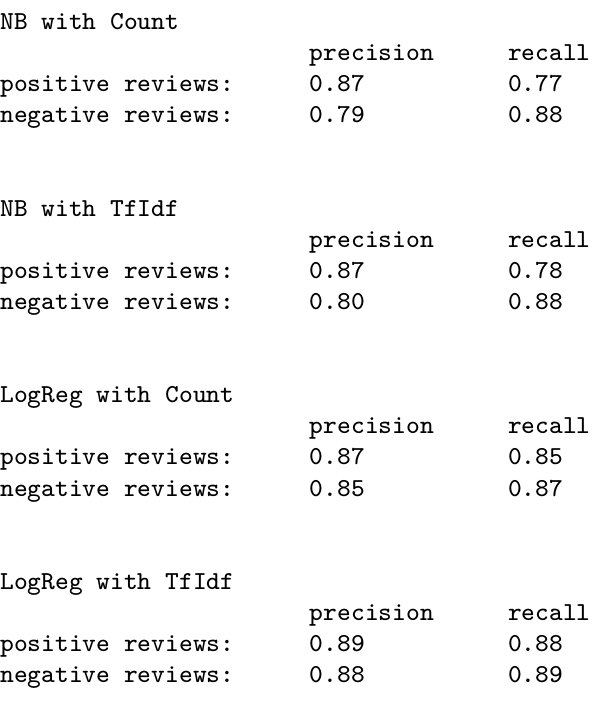
\includegraphics[width=\paperwidth,height=.8\paperheight,keepaspectratio]{imdbsml}}
\end{frame}




\section{Summing up}

\subsection{Revisiting the difference between the dictionary approach and the SML}


\begin{frame}{What \emph{is} our fitted classifier again?}
	Essentially, just a formula 
	
	$$p = \frac{1}{1 + e^{-(\beta_0 + \beta_1 x_1 + \beta_2 x_2 + \ldots + \beta_n x_n)}}$$
	
	where $\beta_0$ is an intercept\footnote{Machine Learning people sometimes call the intercept ``bias'' (yes, I know, that's confusing)}, $\beta_1$ a coefficient for the frequency (or tf$\cdot$ idf score) of some word, $\beta_2$ a coefficient some other word.
	
	If our fitted \emph{vectorizer} contains 5,000 words, we thus have 5,001 coefficients.
	
	\tiny{(for logistic regression in this case, but same argument applies to other classifiers as well)}
	
\end{frame}

\question{But isn't that then essentially very much like a dictionary, except that the words have different weights?}


\begin{frame}{In some sense, yes.}
	\begin{itemize}
		\item But we don't pretend that we can construct the dictionary \emph{a priori}.
		\item It's specifically tailored to our use-case.
		\item The weights are \emph{really} essential here.
	\end{itemize}
	
	\pause
	We \emph{could} print all coefficients-word pairs, but probably it's enough to just look at those with the largest absolute value:
\end{frame}





\begin{frame}{ELI5}
	\makebox[\linewidth]{
		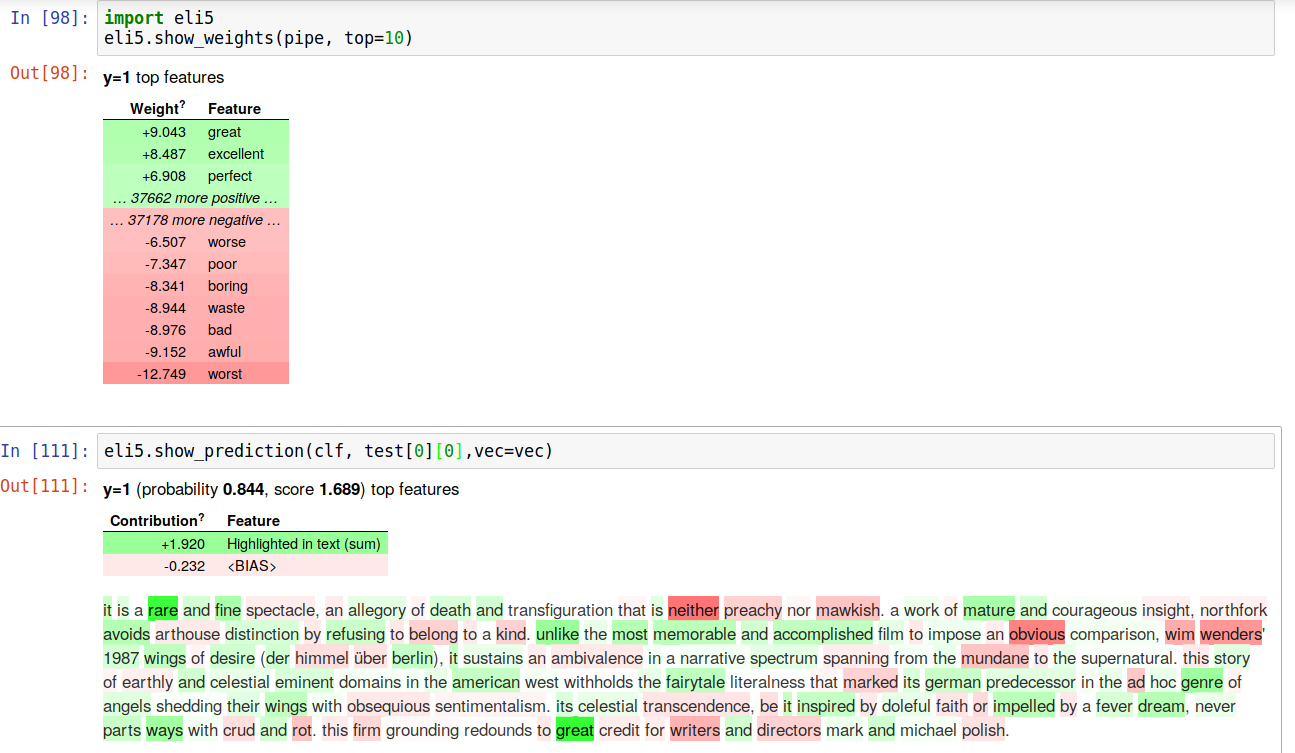
\includegraphics[width=\paperwidth,height=.8\paperheight,keepaspectratio]{eli5}}
\end{frame}

\begin{frame}{ELI5}
	\begin{itemize}
		\item Inspecting \emph{all} coefficients of a ML model usually doesn't make much sense
		\item But that does not mean that we cannot understand how the model makes its predictions
		\item We can look at the most important coefficients
		\item We can look which words in a given text contributed most to its classfication
	\end{itemize}
\end{frame}




\begin{frame}{But have we solved all problems of dictionaries?}
	No.
	
	For instance, the negation and/or intensifier problem.
	
	Possible approaches
	\begin{itemize}
		\item $n$-grams as features
		\item preprocessing (?)
		\item deep learning 
		\item \ldots
	\end{itemize}
	\pause
	
	$\Rightarrow$ \textbf{But ultimately, it's just an empirical question how big the problem is!}
	
	
\end{frame}


\subsection{A note on the input data}

\begin{frame}{The input scikit-learn expects}
	A training dataset consisting of:
	\begin{enumerate}
		\item an array (e.g., a list) of labels (\texttt{y\_train})
		\item a corresponding array (e.g., a list) of feature vectors (\texttt{X\_train})
	\end{enumerate}
	
	A test dataset consisting of:
	\begin{enumerate}
		\item an array (e.g., a list) of labels (\texttt{y\_test})
		\item a corresponding array (e.g., a list) of feature vectors (\texttt{X\_test})
	\end{enumerate}
	
	The feature vectors can be created via a \textit{vectorizer}, but could in principle also just be lists themselves.
	
	We use a lowercase \texttt{y} because it is a onedimensional vector, and an uppercase \texttt{X} because it is a two-dimensional matrix.
\end{frame}


\begin{frame}{The input scikit-learn expects}
	\begin{itemize}
		\item \textbf{It does not matter \emph{how} you create \texttt{y} and \texttt{X}!}
		\item Getting data into the right shape can be as much work (or more) as training the classifier itself
	\end{itemize}
	\pause
	Typical techniques:
	\begin{itemize}
		\item Reading text files from folders into lists of strings (looping over folder contents)
		\item Reading from csv file either directly into lists (\texttt{csv} module) or via pandas
		\item List comprehension to restructure or process data
		\item Potentially, you need to split into train and test dataset yourself (with slicing, or  with scikit-learn itself)
	\end{itemize}
	
	
\end{frame}












%\section{Summing up}

\question{Any questions?}

\begin{frame}{Things to remember}
\begin{itemize}
	\item unsupervised vs supervised
	\item rough understanding of different techniques and when to use them
	\item evaluation metrics (e.g., precision, recall)
\end{itemize}
\end{frame}

\begin{frame}[standout]
	Let's do an exercise!
\end{frame}


\begin{frame}[plain]
	\printbibliography
\end{frame}


\end{document}
